\documentclass[a4paper,14pt]{extarticle}

\usepackage[T2A]{fontenc}
\usepackage[utf8]{inputenc}
\usepackage[russian]{babel}

\usepackage[left=20mm, top=20mm, right=20mm, bottom=20mm]{geometry}
\usepackage{indentfirst}
\usepackage{hyperref}
\usepackage{graphicx}
\usepackage{tikz}
\usepackage{amsmath}
\usepackage{float}
\usetikzlibrary{positioning}

\begin{document}
	
	% ---------------- ТИТУЛЬНЫЙ ЛИСТ ----------------
	{\thispagestyle{empty}
		\begin{center}
			\hfill \break
			\hfill \break
			Министерство образования и науки Российской Федерации\\[3pt]
			Санкт-Петербургский политехнический университет Петра Великого\\[10pt]
			Институт компьютерных наук и кибербезопасности\\[3pt]
			Высшая школа технологий искусственного интеллекта\\[3pt]
			Направление: 02.03.01 «Математика и компьютерные науки»\\[110pt]
			
			\large Техническое задание на курсовую работу\\[5pt]
			\large по дисциплине «Теория графов»\\[5pt]
			\large на тему:\\[5pt]
			\Large \textbf{«Экспертная система определения типа аллергии»}\\[5pt]
			
		\end{center}
		
		\vspace{90pt}
		
		\begin{tabular*}{460pt}{@{\extracolsep{\fill}} l r l}
			Выполнил студент\tabularnewline группы 5130201/40002 & \hspace{55pt} \line(1,0){100} \hspace{-35pt} & Алексеев Л. К.\\
			& \\
			Проверил \tabularnewline преподаватель & \hspace{55pt} \line(1,0){100} \hspace{-35pt} & \hfill Востров А. В. \\
			& \\
			& \\
			& \\
			& \multicolumn{2}{r}{\guillemotleft \line(1,0){30} \guillemotright \line(1,0){100} \, 2026г.}
			
		\end{tabular*} \\
		
		\vfill
		\centering Санкт-Петербург\\
		2026
		\newpage
	}
	
	\tableofcontents
	\newpage
	
	% ---------------- ВВЕДЕНИЕ ----------------
	\section*{Введение}
	\addcontentsline{toc}{section}{Введение}
	
	Целью курсовой работы является разработка экспертной системы, основанной на продукционной модели представления знаний, для определения типа аллергии по симптомам пользователя.  
	
	Система должна работать в среде CLIPS, использовать бинарное дерево решений (не менее четырёх ярусов и тридцати узлов), а также содержать набор продукционных правил, позволяющих классифицировать аллергические реакции.
	
	\newpage
	
	% ---------------- 1. ОБЩИЕ СВЕДЕНИЯ ----------------
	\section{Общие сведения}
	
	Аллергия — это реакция иммунной системы на различные раздражители (аллергены). Тип аллергии определяется по совокупности симптомов: кожные реакции, респираторные проявления, сезонность, контактные факторы и другие признаки.
	
	Экспертная система должна имитировать работу врача‑аллерголога, задавая пользователю вопросы и на основе ответов определяя наиболее вероятный тип аллергии.
	
	\subsection{Цель разработки}
	
	Создать экспертную систему, способную:
	\begin{itemize}
		\item классифицировать тип аллергии по симптомам;
		\item объяснять ход рассуждений (вывод);
		\item работать в интерактивном режиме;
		\item использовать продукционные правила и бинарное дерево решений.
	\end{itemize}
	
	\subsection{Обоснование выбора темы}
	
	Тема соответствует требованиям курсовой работы:
	\begin{itemize}
		\item признаки (симптомы) хорошо формализуются;
		\item большое количество возможных комбинаций симптомов позволяет построить бинарное дерево с числом узлов не менее 30;
		\item продукционные правила естественно описывают процесс медицинской диагностики.
	\end{itemize}
	
	\newpage
	
	% ---------------- 2. ТРЕБОВАНИЯ К СИСТЕМЕ ----------------
	\section{Требования к системе}
	
	\subsection{Функциональные требования}
	
	Экспертная система должна:
	\begin{enumerate}
		\item Запрашивать у пользователя информацию о симптомах и условиях:
		\begin{itemize}
			\item наличие кожной сыпи, зуда, покраснения;
			\item наличие чихания, кашля, слезотечения, насморка;
			\item наличие контакта с животными, пылью, бытовой химией, лекарствами, пищевыми продуктами;
			\item сезонность проявлений (весна, лето, осень, зима, круглогодично).
		\end{itemize}
		\item На основе ответов переходить по бинарному дереву решений.
		\item Применять продукционные правила для вывода диагноза.
		\item Выдавать один из возможных типов аллергии:
		\begin{itemize}
			\item пищевая аллергия;
			\item аллергия на пыльцу (сенная лихорадка);
			\item аллергия на животных;
			\item контактный дерматит;
			\item аллергия на пыль/клещей;
			\item медикаментозная аллергия;
			\item неопределённый тип (недостаточно данных).
		\end{itemize}
		\item Выводить краткое объяснение, какие симптомы и правила привели к результату.
	\end{enumerate}
	
	\subsection{Нефункциональные требования}
	
	\begin{itemize}
		\item Реализация в среде CLIPS версии 6.30 или совместимой.
		\item Использование продукционной модели представления знаний.
		\item Наличие бинарного дерева решений с не менее чем четырьмя ярусами и тридцатью узлами.
		\item Возможность расширения базы знаний новыми правилами без изменения механизма вывода.
	\end{itemize}
	
	\newpage
	
	% ---------------- 3. МОДЕЛЬ ПРЕДСТАВЛЕНИЯ ЗНАНИЙ ----------------
	\section{Модель представления знаний}
	
	\subsection{Продукционная модель}
	
	В качестве модели представления знаний используется продукционная модель. Каждое правило имеет вид:
	
	
	
	ЕСЛИ (условия на симптомы и факты), ТО (вывод о типе аллергии или промежуточный факт).

	
	
	Примеры продукционных правил (на естественном языке):
	
	\begin{itemize}
		\item Если есть кожная сыпь и был контакт с бытовой химией, то предполагается контактный дерматит.
		\item Если есть чихание, слезотечение и симптомы усиливаются весной, то предполагается аллергия на пыльцу.
		\item Если есть кашель и симптомы усиливаются при контакте с животными, то предполагается аллергия на животных.
		\item Если есть отёк и симптомы появились после приёма лекарства, то предполагается медикаментозная аллергия.
	\end{itemize}
	
	\subsection{Структура правила}
	
	Каждое правило в CLIPS будет иметь форму:
	
	\begin{verbatim}
		(defrule имя-правила
		(условие-1)
		(условие-2)
		...
		=>
		(assert (новый-факт ...)))
	\end{verbatim}
	
	\subsection{Рабочая память}
	
	Рабочая память системы будет содержать:
	\begin{itemize}
		\item факты о симптомах пользователя;
		\item факты о контекстных условиях (сезон, контакт с аллергенами);
		\item промежуточные выводы;
		\item финальный диагноз.
	\end{itemize}
	
	\newpage
	
	% ---------------- 4. БИНАРНОЕ ДЕРЕВО РЕШЕНИЙ ----------------
	\section{Бинарное дерево решений}
	
	Для реализации логического вывода используется бинарное дерево решений. Каждый внутренний узел дерева соответствует вопросу (условию), а каждая дуга — ответу «да» или «нет». Листья дерева соответствуют возможным типам аллергии или состоянию «недостаточно данных».
	
	Ниже приведён фрагмент дерева решений (полная версия будет расширена до не менее 30 узлов).
	
	\begin{figure}[H]
		\centering
		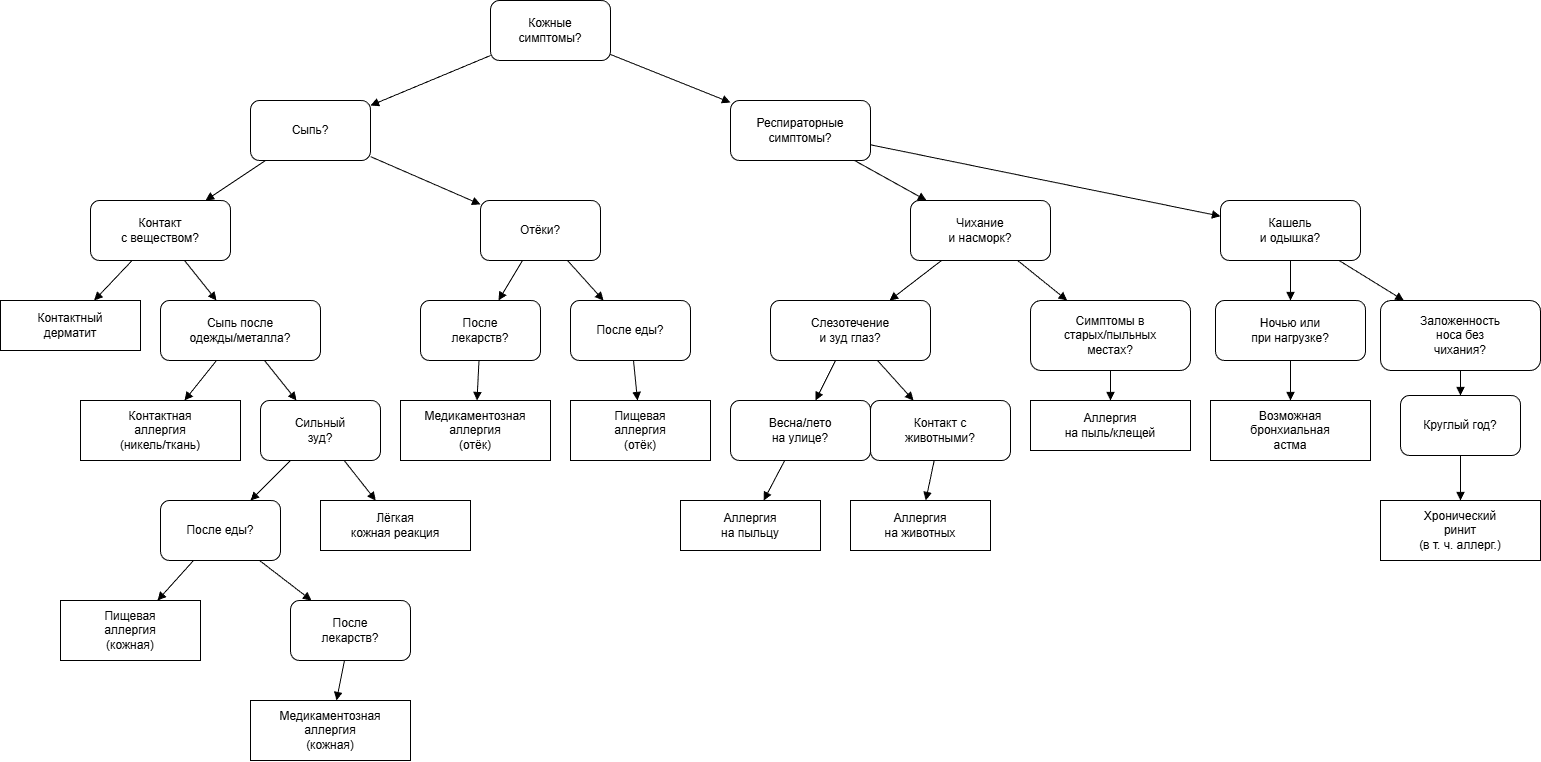
\includegraphics[width=\textwidth]{Tree_allergy.png}
		\caption{Бинарное дерево решений для определения типа аллергии}
	\end{figure}
	
	
	
	
	Полное дерево будет дополнено дополнительными вопросами (например, о времени появления симптомов, связи с приёмом пищи, лекарств, сменой помещения и т. д.), чтобы удовлетворить требование по минимальному числу узлов.
	
	\newpage
	
	% ---------------- 5. СТРУКТУРА ПРОГРАММЫ CLIPS ----------------
	\section{Структура программы в среде CLIPS}
	
	\subsection{Факты и шаблоны}
	
	В системе предполагается использование следующих типов фактов:
	
	\begin{itemize}
		\item факты о симптомах: \verb|(симптом чихание)|, \verb|(симптом зуд)| и т. п.;
		\item факты о контактах: \verb|(контакт животные)|, \verb|(контакт бытовая-химия)|;
		\item факты о сезоне: \verb|(сезон весна)|, \verb|(сезон круглогодично)|;
		\item факт о диагнозе: \verb|(диагноз пищевая)| и т. д.
	\end{itemize}
	
	Примеры шаблонов:
	
	\begin{verbatim}
		(deftemplate симптом
		(slot имя))
		
		(deftemplate контакт
		(slot тип))
		
		(deftemplate сезон
		(slot значение))
		
		(deftemplate диагноз
		(slot тип))
	\end{verbatim}
	
	\subsection{Пример продукционных правил}
	
	\begin{verbatim}
		(defrule правило-пыльца
		(симптом (имя чихание))
		(симптом (имя слезотечение))
		(сезон (значение весна))
		=>
		(assert (диагноз (тип пыльца))))
	\end{verbatim}
	
	\begin{verbatim}
		(defrule правило-контактный-дерматит
		(симптом (имя сыпь))
		(контакт (тип бытовая-химия))
		=>
		(assert (диагноз (тип контактный-дерматит))))
	\end{verbatim}
	
	\subsection{Механизм логического вывода}
	
	В системе используется прямой вывод (forward chaining). При добавлении новых фактов (ответов пользователя) активируются правила, условия которых удовлетворены, и в рабочую память добавляются новые факты, в том числе факт о диагнозе.
	
	\newpage
	
	% ---------------- 6. ИНТЕРФЕЙС СИСТЕМЫ ----------------
	\section{Интерфейс системы}
	
	Интерфейс предполагается консольным (текстовым):
	
	\begin{itemize}
		\item система задаёт пользователю вопросы вида «Есть ли у вас чихание? (да/нет)»;
		\item пользователь вводит ответы «да» или «нет»;
		\item на основе ответов формируются факты в рабочей памяти;
		\item после завершения опроса система выводит:
		\begin{itemize}
			\item предполагаемый тип аллергии;
			\item краткое объяснение (какие симптомы и правила привели к выводу).
		\end{itemize}
	\end{itemize}
	
	При необходимости интерфейс может быть расширен до графического (через интеграцию CLIPS с другими языками), но в рамках данного ТЗ достаточно текстового режима.
	
	\newpage
	
	% ---------------- ЗАКЛЮЧЕНИЕ ----------------
	\section*{Заключение}
	\addcontentsline{toc}{section}{Заключение}
	
	В данном техническом задании сформулированы цели, требования и структура экспертной системы для определения типа аллергии. Определены модель представления знаний (продукционная модель), структура бинарного дерева решений, формат фактов и правил в среде CLIPS, а также общие подходы к тестированию и взаимодействию с пользователем.
	
	Реализация системы в соответствии с данным ТЗ позволит получить работоспособную экспертную систему, удовлетворяющую требованиям курсовой работы по дисциплине «Теория графов».
	
\end{document}
